\documentclass{mmposter}

\colorlet{CEmphasis1}{clustercassis}
\colorlet{CEmphasis2}{clusterblue}

\usepackage{lipsum}
\usepackage{blindtext}
\usepackage{tikz}
\usepackage{amsmath}
\usepackage{hyperref}
\hypersetup{
	colorlinks,
	citecolor=black,
	urlcolor=CEmphasis1,
}

\title{Improving Interoperability\\in Scientific Computing\\via MaRDI Open Interfaces}
\authors{Contributors:
	Dmitry I.\ Kabanov, Stephan Rave, Mario Ohlberger
}
\renewcommand{\refname}{References}

\newcommand{\OIF}{\textsc{MaRDI Open Interfaces}\xspace}

\newcounter{hilfszaehler}

\graphicspath{{./assets/}}

\begin{document}
\bibliographystyle{plain}

\maketitle

\section*{Summary}
We develop \OIF{} to improve interoperability of scientific software.

\begin{objectives}
  \item Develop library that passes data between languages automatically
  \item Develop interfaces for typical numerical problems
  such as optimization and integration of differential equations
  \item Spread information about open interfaces to encourage
  scientific-computing community to program against these interfaces.
\end{objectives}

\section*{Architecture}
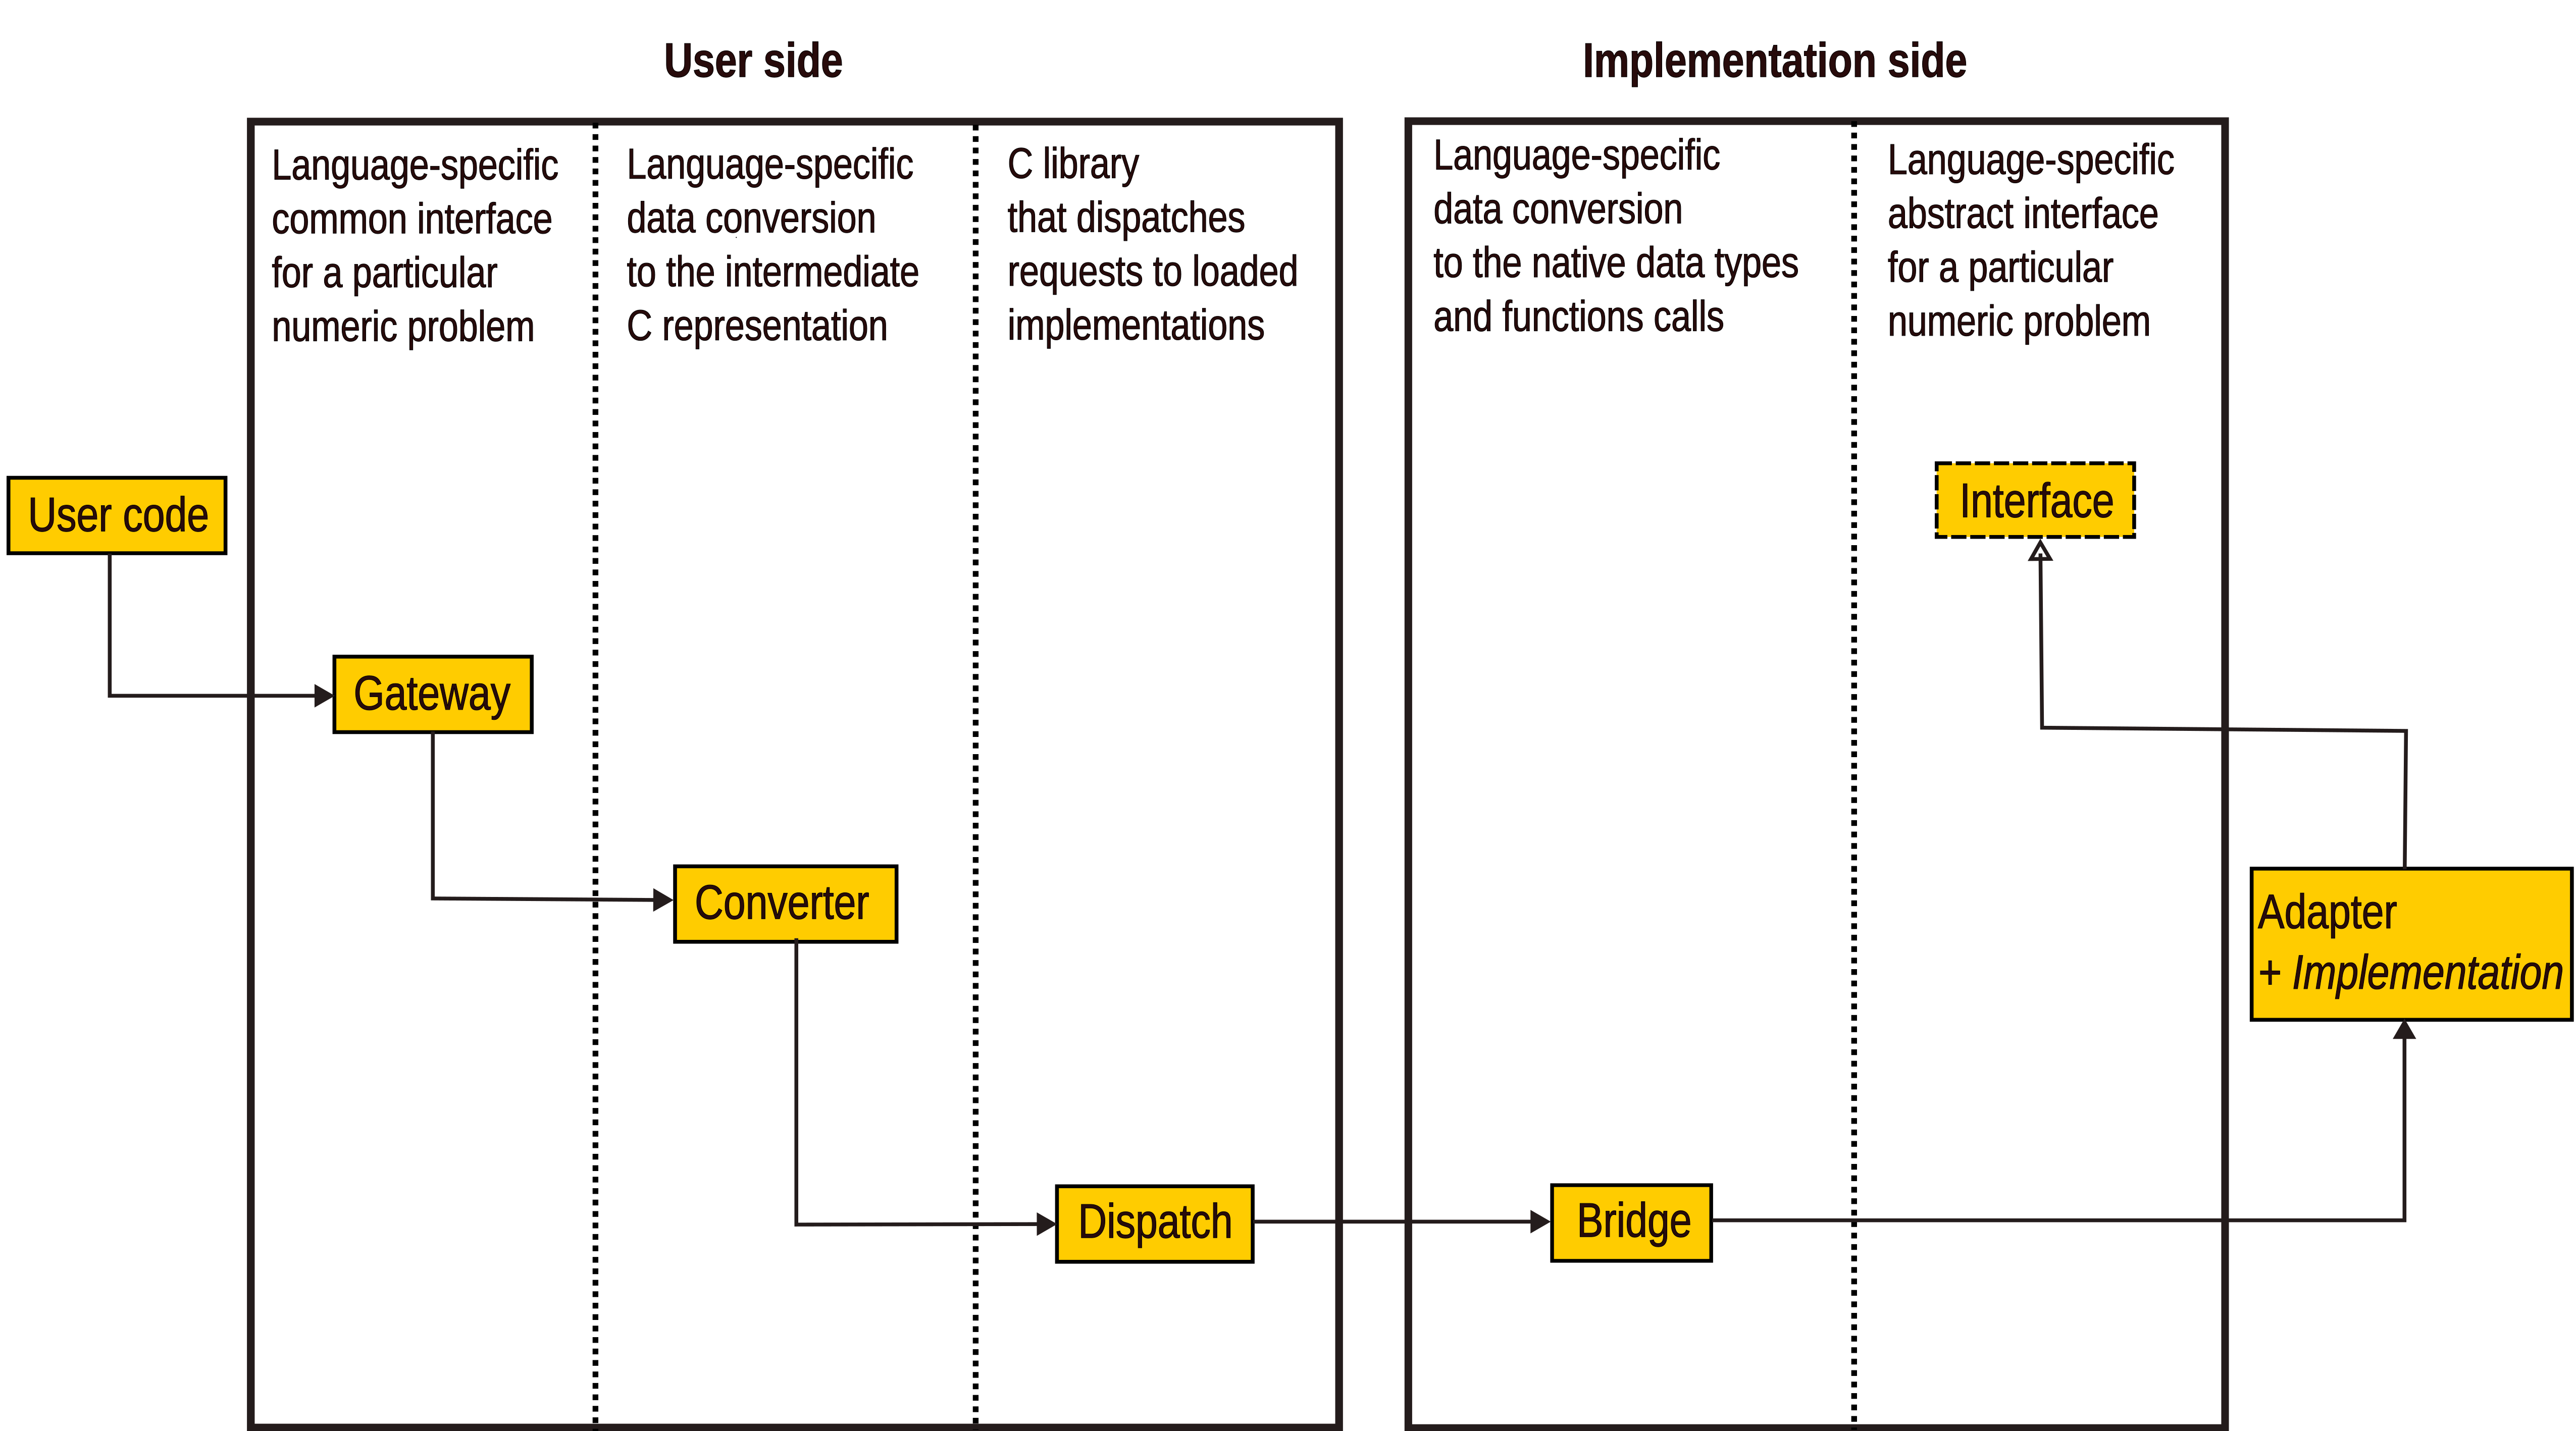
\includegraphics[width=\columnwidth]{arch.png}

\newpage

\section*{Example usage}
\lipsum[2]

\section*{Conclusions}
\lipsum[3]

\section*{Connections to other MaRDI subprojects}

\begin{itemize}[align=left]
  \item[\color{CEmphasis1}M2.3:] Benchmarking of MOR software is potentially
    easier using \OIF{}.
  \item[\color{CEmphasis1}M?.?:] Tool that helps with reproducibility
    by ``containerization''.
\end{itemize}

\begin{thebibliography}{1}
  \setlength{\itemsep}{1pt}
  \setlength{\parskip}{1.5pt}

  \scriptsize{

  \bibitem[1]{PyMOR}
  Ren{\'{e}}, M., Rave, S., and Schindler, F.
  \newblock pyMOR -- Generic Algorithms and Interfaces for Model Order Reduction, 2016.
  \newblock doi:10.1137/15m1026614.
  }
\end{thebibliography}

\end{document}
